% Use wide margins, but not quite so wide as fullpage.sty
\documentclass[11pt]{article}   
\marginparwidth 0.5in 
\oddsidemargin 0.25in 
\evensidemargin 0.25in 
\marginparsep 0.25in
\topmargin 0.25in 
\textwidth 6in \textheight 8 in
% That's about enough definitions

% multirow allows you to combine rows in columns
\usepackage{multirow}
% tabularx allows manual tweaking of column width
\usepackage{tabularx}
% longtable does better format for tables that span pages
\usepackage{longtable}
\usepackage{listings}
\usepackage{graphicx}
\graphicspath{ {./images/} }

\begin{document}
% this is an alternate method of creating a title
%\hfill\vbox{\hbox{Gius, Mark}
%       \hbox{Cpe 456, Section 01}  
%       \hbox{Lab 1}    
%       \hbox{\today}}\par
%
%\bigskip
%\centerline{\Large\bf Lab 1: Security Audit}\par
%\bigskip
\author{Kinner Parikh}
\title{Project 5}
\maketitle
\begin{center}
    CMPEN 331 - 001
\end{center}

\newpage

\section{Code}


\ttfamily
\lstinputlisting{Modules.v}

\newpage

\ttfamily
\lstinputlisting{Modules.v}

\newpage

\ttfamily
\lstinputlisting{testbench.v}

\rmfamily
\section{Images}

\begin{center}
    \underline{Timing Waveform}

    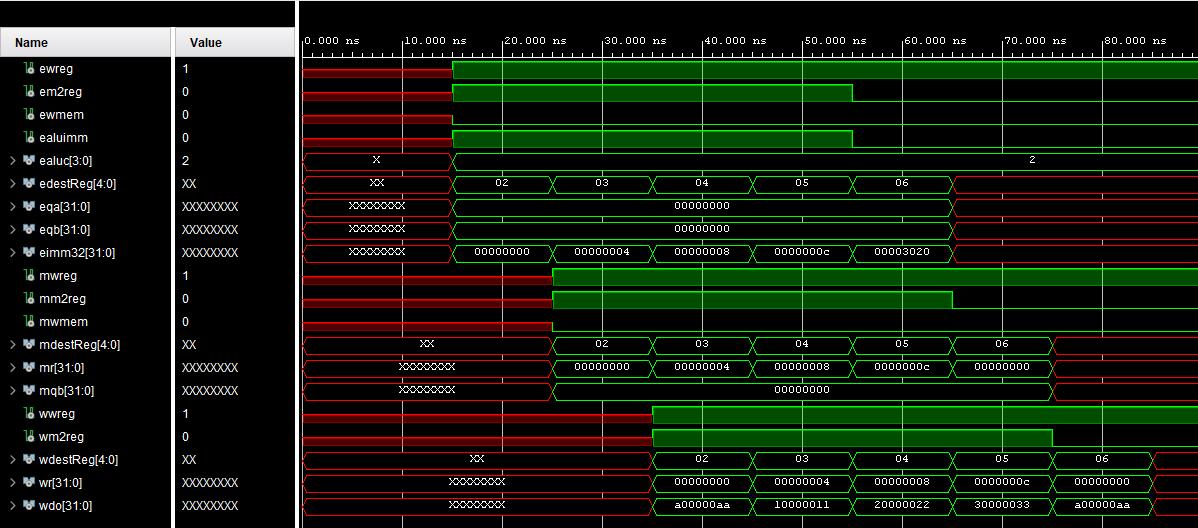
\includegraphics[width = 1\textwidth]{waveform.png}
    
    \newpage

    \underline{Schematic}

    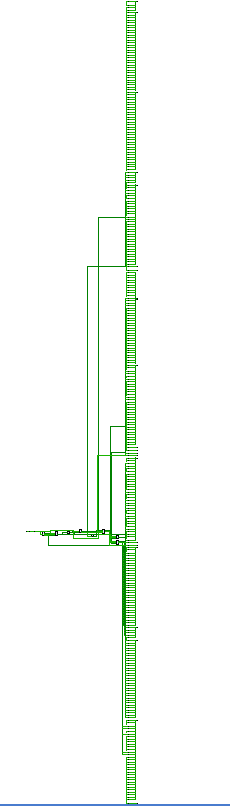
\includegraphics[scale = 1]{schematic.png}

    \newpage

    \underline{I/O Planning}

    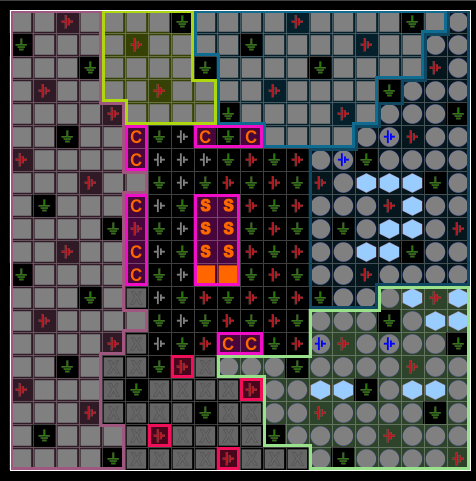
\includegraphics[width = 1\textwidth]{ioplan.png}
    \newpage

    \underline{Floor Planning}

    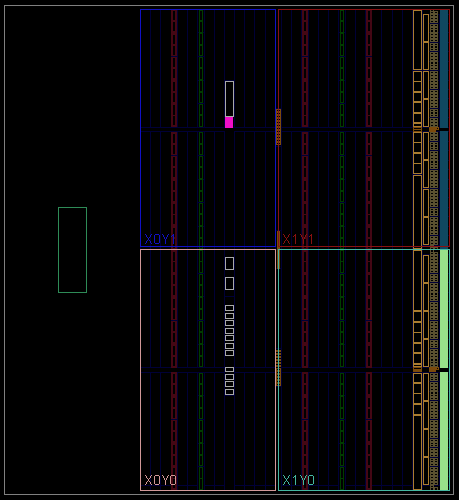
\includegraphics[width = 1\textwidth]{floorplan.png}


\end{center}

\end{document}